\newsavebox{\boxcc}
\Savebox{\boxcc}{
\hspace{-0.25cm}
\begin{minipage}[l]{\columnwidth}
\begin{lstlisting}[style=conescframe]
context group BaseStationG {
*\lstnote{layereddef}* layered command void report(msg_t msg);
}implementation {
*\lstnote{contexts}* contexts Reachable,
*\lstnote{isdefault}*          Unreachable is default,
*\lstnote{iserror}*          MyErrorC is error;
 components Routing, Logging;
 Reachable.Collection -> Routing;
 Unreachable.DataStore -> Logging;}
\end{lstlisting}
\end{minipage}
}
\newsavebox{\boxbscm}
\Savebox{\boxbscm}{
\hspace{-0.25cm}
\begin{minipage}[l]{\columnwidth}
\begin{lstlisting}[style=conescframe]
module BaseStationContextManager {
 uses context group BaseStationG;
}implementation {
 event msg_t Beacon.receive(msg_t msg) {
*\lstnote{actBS}*  activate BaseStationG.Reachable;
  call BSReset.stop(); 
  call BSReset.startOneShot(TIMEOUT);}
 event void BSReset.fired() {
*\lstnote{actNoBS}*  activate BaseStationG.Unreachable;}}
\end{lstlisting}
\end{minipage}
}
\newsavebox{\boxc}
\Savebox{\boxc}{
\hspace{-0.25cm}
\begin{minipage}[l]{\columnwidth}
\begin{lstlisting}[style=conescframe]
context Unreachable {
*\lstnote{dependence}* transitions Reachable iff ActivityG.Running;
 uses interface DataStore;
}implementation {
*\lstnote{activatedUnreachable}* event void activated(){//...}
*\lstnote{deactivatedUnreachable}* event void deactivated(){//...}
*\lstnote{checkUnreachable}* command bool check(){//...}
 layered command void report(msg_t msg){
*\lstnote{layeredimp}*  call DataStore.deposit(msg);}}
\end{lstlisting}
\end{minipage}
}
\newsavebox{\boxirc}
\Savebox{\boxirc}{
\hspace{-0.25cm}
\begin{minipage}[l]{\columnwidth}
\begin{lstlisting}[style=conescframe]
context Reachable {
 uses interface Collection;
 uses context group BatteryG; 
}implementation {
*\lstnote{activated}* event void activated(){ 
  call GPS.stop();}
*\lstnote{deactivated}* event void deactivated(){//...}
*\lstnote{check}* command bool check(){
  return call BatteryG.getContext() == BatteryG.Normal;}
 layered command void report(msg_t msg){
*\lstnote{layeredimp2}*  call Collection.send(msg);}}
\end{lstlisting}
\end{minipage}
}
\newsavebox{\boxlc}
\Savebox{\boxlc}{
\hspace{-0.25cm}
\begin{minipage}[l]{\columnwidth}
\begin{lstlisting}[style=conescframe]
context Low {
*\lstnote{triggers}* triggers BaseStationG.Unreachable;
}implementation {//...}
\end{lstlisting}
\end{minipage}
}
% \newsavebox{\boxmc}
% \Savebox{\boxmc}{
% \hspace{-0.25cm}
% \begin{minipage}[l]{\columnwidth}
% \begin{lstlisting}[style=conescframe]
% configuration ApplicationC {
% }implementation {
% *\lstnote{declaration}* components BaseStationG, Application;
%  //...
% *\lstnote{wiring}* Application.BaseStationG -> BaseStationG;}
% \end{lstlisting}
% \end{minipage}
% }
\newsavebox{\boxmm}
\Savebox{\boxmm}{
\hspace{-0.25cm}
\begin{minipage}[l]{\columnwidth}
\begin{lstlisting}[style=conescframe]
module User {
*\lstnote{cgdecl}* uses context group BaseStationG;
}implementation {
 event void Timer.fired() {
*\lstnote{calling}*  call BaseStationG.report(msg);}
*\lstnote{eventCC}* event void BaseStationG.contextChanged(context_t con) {
*\lstnote{concheck}*  if(con == BaseStationG.Reachable) // DO SOMETHING...}}
\end{lstlisting}
\end{minipage}
}
\newsavebox{\boxnmc}
\Savebox{\boxnmc}{
\hspace{-0.25cm}
\begin{minipage}[l]{\columnwidth}
\begin{lstlisting}[style=conescframe]
context NotMoving {
*\lstnote{transitions}* transitions Resting;
}implementation {//...}
\end{lstlisting}
\end{minipage}
}
\vspace{-0.09in}
\section{ConesC}\label{sec:conesc}

% \conesc provides a design-time support for developing a self-adaptive software,
% which alternates its behavior at run-time including catching and handling
% errors. Along with this, our approach provides a deep modularization, since
% behavioral variations are encapsulated into different modules. The latter, as we
% show in Sec.~\ref{sec:evalcomp}, are highly decoupled, which enhances code
% readability and re-usability as well as debugging and developing processes.

We illustrate how we render the concepts in
Section~\ref{sec:appdesign} within \conesc: our own context-oriented
extension to nesC.  We describe a notion of context module and
configuration in Section~\ref{subsec:components}, and discuss in
Section~\ref{subsec:usage} how programmers use these constructs to
specify an application's adaptive behavior.
Section~\ref{subsec:usage} describes how \conesc programmers may deal
with unforeseen context evolutions.

\subsection{Contexts and Context Groups}\label{subsec:components}

\putsnippet{
 caption=Context group in \conesc.,
 label=fig:ccc,
 boxname=boxcc
}

Context groups in \conesc extend the standard nesC
configurations. Programmers use context groups to to declare layered
functions and the contexts providing the corresponding behavioral
variations depending on the situation. 

Fig.~\ref{fig:ccc} shows an example for the \emph{Base-station}
group. A layered \code{report} function is declared on
line~\lstref{layereddef} by using the keyword \code{layered}. The
contexts providing the necessary behavioral variations are specified
following the keyword \code{contexts} on line~\lstref{contexts}. In
this case, programmers define two such contexts, depending on
base-station reachability. The \code{is default} modifier, shown on
line~\lstref{isdefault} indicates what context is active at
startup. The next \code{is error} modifier on line~\lstref{iserror}
declares context \code{ErrorC} as an \emph{error} context, which
programmers may optionally use to handle errors during the execution,
as we discuss in Section~\ref{subsec:rules}. If an error context is
not declared, it is generated automatically.

\putsnippet{
 caption=\emph{Reachable} context.,
 label=fig:irc,
 boxname=boxirc
}

\putsnippet{
 caption=\emph{Unreachable} context.,
 label=fig:cc,
 boxname=boxc
}

The individual contexts in \conesc extend the standard nesC modules by
providing context-dependent implementations of layered function
declared in context groups. Only one context at a time can be
\emph{active} in a group, meaning only one context at a time can
provide the implementation of a given layered function.

For example, Fig.~\ref{fig:irc} and~\ref{fig:cc} show \conesc snippets
for the \emph{Reachable} and \emph{Unreachable} contexts referenced in
Fig.~\ref{fig:ccc}. They provide different implementations for
\code{report} dependsing on the situation. If the base-station is
\emph{Reachable}, this the corresponding context is active, the code
transmits the message to the base-station, as in
line~\lstref{layeredimp2} of Fig~\ref{fig:irc}. Differently, the code
deposits a message in local memory as in line~\lstref{layeredimp} of
Fig.~\ref{fig:cc}.

Developer may need to specify operations upon activating a context,
such as initialization of variables or enabling/disabling hardware
modules. For example, on entering the \emph{Reachable} context,
programmers may decide to disable the GPS sensor, as location
information can be inferred from the (static)
base-station. Programmers specify this functionality within the body
of a predefined \code{activated} event, as in
line~\lstref{activatedUnreachable} of Fig.~\ref{fig:irc}. Similarly,
programmers may specify clean-up operations within \code{deactivated}
events, as in line~\lstref{deactivatedUnreachable} of
Fig.~\ref{fig:irc}.  Providing an implementation for these events,
however, is not mandatory.

\subsection{Execution}\label{subsec:usage}

% Context groups encaspulate behavioral variations sharing some common
% characteristic or related to the same funcitonality. Within the
% \emph{Base-station} group of Fig.~\ref{fig:ccc}, for example,
% programmers activate different behavioral variations for function
% \code{report} depending on base-station reachability. 

\putsnippet{
 caption=Base-station context manager.,
 label=fig:bscm,
 boxname=boxbscm
}

Fig.~\ref{fig:bscm} shows an sample snippet of code to detect and to
activate the proper context in the base-station example. Programmers
can, anywhere in the code, trigger explicit changes between contexts
in a group. This is as simple as using the \code{activate} keyword
followed by a full context name. In this fragment of code, the
\emph{Reachable} context is activated on line~\lstref{actBS} as soon
as a beacon from the base station is received. Should the timeout
expire with no more beacons received, context \emph{Unreachable} is
activated on line~\lstref{actNoBS}. Either context change results in a
different context-dependent implemenation of \code{report} to be
activated.

\putsnippet{
 caption=User module.,
 label=fig:mm,
 boxname=boxmm
}

Modules using layered functions perform function calls transparently
w.r.t. the available contexts and, most importantly, independently of
what context is active at a given moment. Fig.~\ref{fig:mm} shows one
such example where no explicit references appear to which and how many
behavrioal variations exist for function \code{report()}. Following
the indication that context group \emph{BaseStationG} is used, as
specified on line~\lstref{cgdecl}, the call to function \code{report}
on line~\lstref{calling} refers to the context group and not to the
individual contexts. The net advatnage is that the use of
context-dependent functionality and the functionality to manage
context detection and activation are fully decoupled and can thus live
separate, even in a different modules.


Nevertheless, should the programmers of user module need to find out
about context changes, a predefined event~\code{contextChanged} is
fired corresponding to every context change, as shown on line~\lstref{eventCC} in
Fig.~\ref{fig:mm}. % This event can be caught
% and handled, as it is shown on the line~\lstref{eventCC} in
% Fig.~\ref{fig:mm}, but it is not mandatory though.
Within the event handler, programmers can access costant values in a
context group that our translator automatically egnerates, as
described in Section~\ref{sec:translator}, to find out what context
was activated and to react accordingly, as shown on
line~\lstref{concheck}.


% This section shows how ConesC can be used to invoke a behavioral
% variation. Here we describe one aspect of an application's behavioral variation,
% which is related to the Base Station availability. As it was mentioned before,
% if a node receives a beacon from the Base Station it activates the \emph{Reachable}
% context, and the \emph{Unreachable} context in case of timeout.
% Since the behavioral variation is encapsulated in a context group \emph{BaseStationG},
% a developer may not care about the context implementation and use a context group
% Tiny fix.to change a behavior of the application at run-time. Fig.~\ref{fig:mc} depicts the main
% configuration, where the base station group is declared on line~\lstref{declaration} and wired
% as a standard component afterward on the line~\lstref{wiring}.

% \putsnippet{
%  caption=Main configuration.,
%  label=fig:mc,
%  boxname=boxmc
% }

\subsection{Transition Rules}\label{subsec:rules}

In ConesC every context transition implies several checking stages, which are displayed in
Fig.~\ref{fig:ad}, such as: possibility of the transition, dependencies check and conditions
check. The successful check allows to continue a transition, while the failure leads either to
the canceling of the transition or to activation of the \emph{error} context. The latter is generated
automatically unless declared in a \emph{context group} by using the key-word \emph{is error},
as shown in Fig.~\ref{fig:ccc} on line~\lstref{iserror}.

\putfigure{ caption=Activation diagram.,label=fig:ad}{
 \centering
 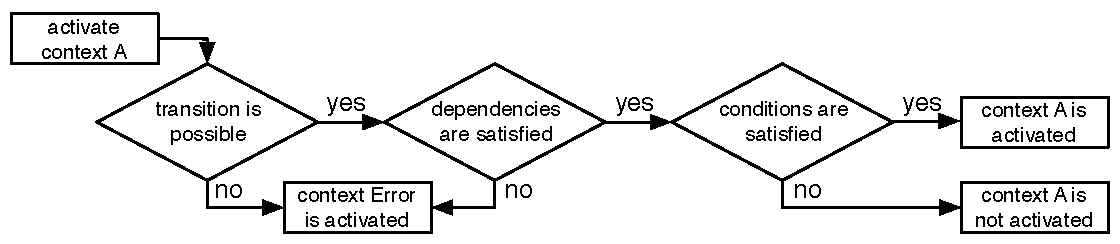
\includegraphics[width=\columnwidth]{pdf/activation_diagram}
}

In our scenario, which is displayed on a figure~\ref{fig:wtd}, within \emph{Activity} group a
transition from \emph{NotMoving} to \emph{Resting} is only possible, and it is checked
by the first conditional chose displayed on a figure~\ref{fig:ad}.
Since each transition is governed by a separate rule, it is declared in a context component as shown
on line~\lstref{transitions} in figure~\ref{fig:nmc}. Here key-word \emph{transitions}
indicates the contexts a transition can be performed to. An attempt to initiate
a transition to the context, which is not declared in a given active context, leads to an error context
activation, since this kind of transitions is not possible.

\putsnippet{
 caption=NotMoving context.,
 label=fig:nmc,
 boxname=boxnmc
}

Despite the application's  functionality is split into isolated pieces by \emph{context groups},
there may exist relations among them. For example, within the 
\emph{Health conditions} group a transition from \emph{Healthy} to \emph{Diseased} is only
make sense if an animal is \emph{Resting} or \emph{NotMoving}. These inter-group
relations are covered in our context-oriented language by context dependencies,
which are checked in the second conditional chose on a figure~\ref{fig:ad}. In
ConesC dependencies are declared as it is shown on the line~\lstref{dependence}
in Fig.~\ref{fig:cc}. In \emph{transitions} section a context name followed by a
key-word \emph{iff} and a full name of another context means that
the transition will only be executed if the latter context is active. Should the
rule with dependency be violated, a transition to an error context will be triggered.

The last conditional chose displayed on a figure~\ref{fig:ad} is used for soft rules, violation of
which does not affect the execution of a program. For example, context~\emph{Running} is
activated if the difference between two GPS readings is relatively large, but it may be due to noise.
To make sure false positives are avoided, developers may want to check
readings of an accelerometer. Another example includes an energy saving scenario,
when a programmer may want to activate~\emph{Reachable} context only if a battery is
in~\emph{Normal} state, as shown in Fig.~\ref{fig:wtd}.
Violation of mentioned rules is a common situation and should not lead to an error state.
To this end, ConesC provides a \emph{check()} command, sample implementation of which is
displayed on the line~\lstref{check} in Fig.~\ref{fig:irc}. It is not mandatory to implement this
command, but should it return \emph{FALSE}, an initiated context transition does not occur,
a context is not activated and a system remains in the previous state.
This approach allows one not to think about conditions a transition taking
place in, but foresee possible inconsistencies.

Other types of inter-group relations imply automatic triggering of context
transition. Considering \emph{Battery} group in our example, we can notice that
for further energy saving developers may want to trigger a transition to
\emph{Unreachable} context within the \emph{Base Station} group as long as
\emph{Low} context is active. Our design allows one to do that by declaring a
\emph{triggers} section, as shown on the line~\lstref{triggers} in Fig.~\ref{fig:lc}.
The same checks apply to automatic transitions.

\putsnippet{
 caption=Low context.,
 label=fig:lc,
 boxname=boxlc
}



%%% Local Variables: 
%%% mode: latex
%%% TeX-master: "bare_conf"
%%% End: 
